% TEXINPUTS=.:$HOME/git/bvtex: latexmk  -pdf <main>.tex
\documentclass[xcolor=dvipsnames]{beamer}

\input{defaults}
\input{beamer/preamble}

\setbeamertemplate{navigation symbols}{}
% \setbeamertemplate{background}[grid][step=1cm]

\usepackage{siunitx}
\usepackage{xmpmulti}
\usepackage[export]{adjustbox}

\usepackage[outline]{contour}
\usepackage{tikz}
\usetikzlibrary{shapes.geometric, arrows}
\usetikzlibrary{positioning}

\definecolor{bvtitlecolor}{rgb}{0.98, 0.92, 0.84}
\definecolor{bvoutline}{rgb}{0.1, 0.1, 0.1}

\renewcommand{\bvtitleauthor}{Brett Viren}
\renewcommand{\bvtit}{LARF}
\renewcommand{\bvtitle}{\LARGE \textbf{LArTPC Detector Response Calculations}\\Using \textbf{B}oundary \textbf{E}lement \textbf{M}ethod}
\renewcommand{\bvevent}{$\mu$Boone Sim\\9 Aug 2016}
\renewcommand{\bvbeamerbackground}{}

\newcommand{\microboone}{MicroBooNE\xspace}


\begin{document}
\input{beamer/title.tex}

\begin{frame}[fragile]
  \frametitle{Boundary Element Method (BEM) Overview}
  \begin{enumerate}  \footnotesize
  \item Discretize (mesh) boundary electrode \textbf{surfaces}.
  \item Define (Dirichlet) scalar potential on each mesh element (triangle).
  \item Fit (Neumann) surface-normal boundary field.
  \item Integrate Laplace equation $\nabla^2\phi=0$, evaluate at boundary.
  \item Evaluate solution at points in the volume.
  \end{enumerate}

  \vfill

  \footnotesize

  Compare BEM and FEM:

  \begin{center}

    \begin{tabular}[h]{rcc}
      & BEM & FEM \\
      \hline
      domain: & 2D surface mesh & 3D volume mesh \\
      easy: & away from surface & near to surface \\
      fits: & boundary-normal field & volumetric field \\
      eval: & arb. volume point & volume mesh points \\
      \hline
      both: & \multicolumn{2}{c}{CPU and memory intensive, limited geometries} \\
      external: & \multicolumn{2}{c}{stepping and averaging current responses} \\
    \end{tabular}
  \end{center}

\end{frame}

\begin{frame}
  \frametitle{General Calculation Overview}
  High-level steps:
  \begin{itemize}
  \item Drift fields: $\phi_{drift} \to \vec{E}_{drift} \to \mu \to \vec{v}_{drift} \to$ \textbf{paths}: $\{p\}$
    \begin{itemize}\footnotesize
    \item $\vec{v}_{drift} = \mu(E_{drift}) \vec{E}_{drift}(\vec{r}(t))$
    \item Get path $\vec{r}_p(t)$ by stepping through velocity field $\vec{v}_{drift}$.
    \end{itemize}

  \item Shockley-Ramo ``\textbf{weighting}'' potential for electrode $k$
    \begin{itemize}\footnotesize
    \item $\phi_{weight,k} \to \vec{E}_{weight,k}$
    \item Electrode $k$ at 1V, all others at 0V.
    \end{itemize}
  \item \textbf{Current on wire} $k$ due to charge moving along path $p$: 
    \begin{itemize}\footnotesize
    \item $i_{k,p}(t) = q \vec{E}_{weight,k} \cdot \vec{v}_{drift}|_p$
    \end{itemize}
  \item \textbf{Response function} for wire $k$ is average over paths: 
    \begin{itemize}\footnotesize
    \item $<i_{k}(t)> = \frac{1}{N}\sum_{p=1}^N i_{k,p}(t)$
    \end{itemize}
  \end{itemize}
  \vfill
  \footnotesize
  $\rightarrow$ for now: paths start on 1mm grid, 16mm in front of
  U-plane, 

  $\rightarrow$ response is average over paths in half-pitch ``wire region''
\end{frame}

\begin{frame}
  \frametitle{Wire Meshes}

  \footnotesize

  \begin{columns}
    \begin{column}{0.3\textwidth}
      \begin{center}
        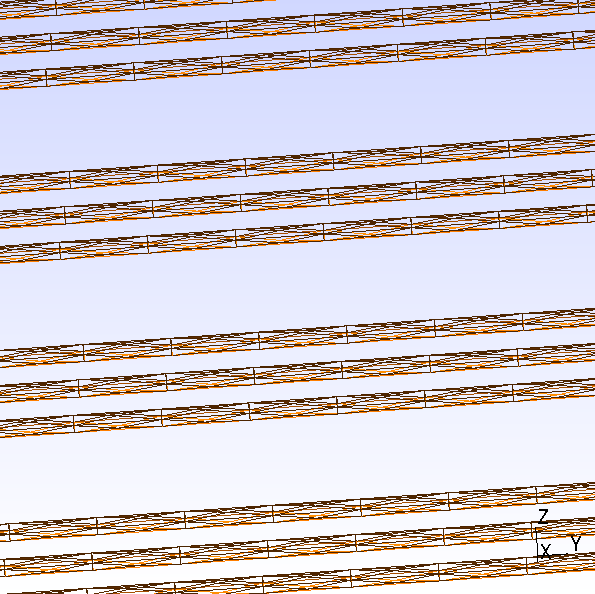
\includegraphics[height=0.4\textheight]{parallel-mesh.png}      
        
        ``Parallel'':\\3mm pitch and gap\\all wires parallel
      \end{center}
    \end{column}
    \begin{column}{0.3\textwidth}
      \begin{center}
        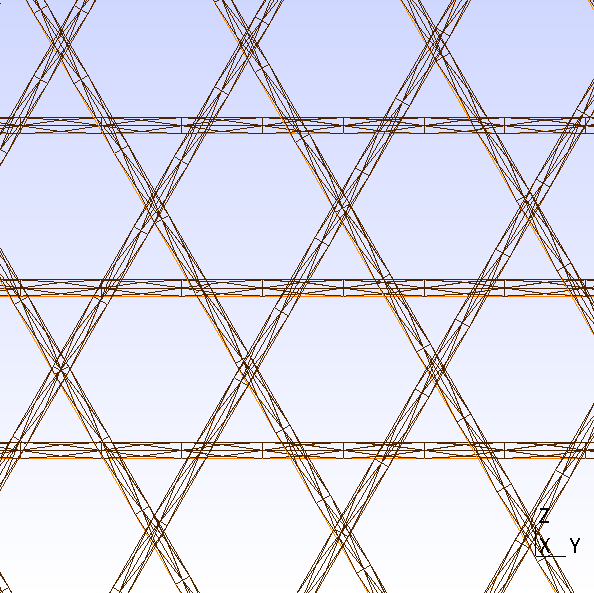
\includegraphics[height=0.4\textheight]{uboone-mesh.png}      

        ``MicroBooNE'':\\3mm pitch and gap\\$60^\circ$ angles for U/V.
      \end{center}
    \end{column}
    \begin{column}{0.3\textwidth}
      \begin{center}
        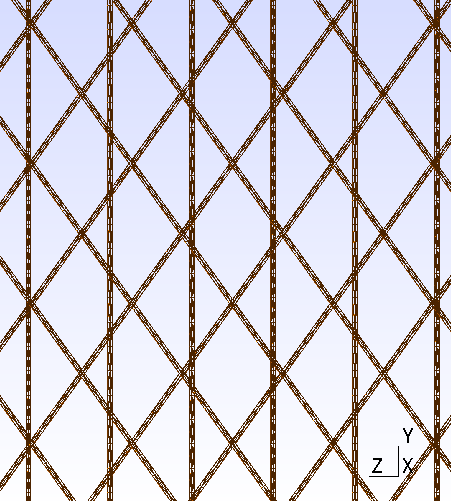
\includegraphics[height=0.4\textheight]{dune-mesh.png}      

        ``DUNE'':\\5mm pitch and gap\\$35.7^\circ$ angles for U/V.
      \end{center}
    \end{column}
  \end{columns}

  \vspace{4mm}

  \begin{itemize}
  \item ``Parallel'' used to reproduce 2D calculations. 
  \item Geometry parameterized to facilitate exploring different configurations.
  \end{itemize}

\end{frame}


\begin{frame}
  \frametitle{Parallel Wires - Slice Through Weighting Potentials}
  \begin{columns}
    \begin{column}{0.5\textwidth}
      \begin{center}
        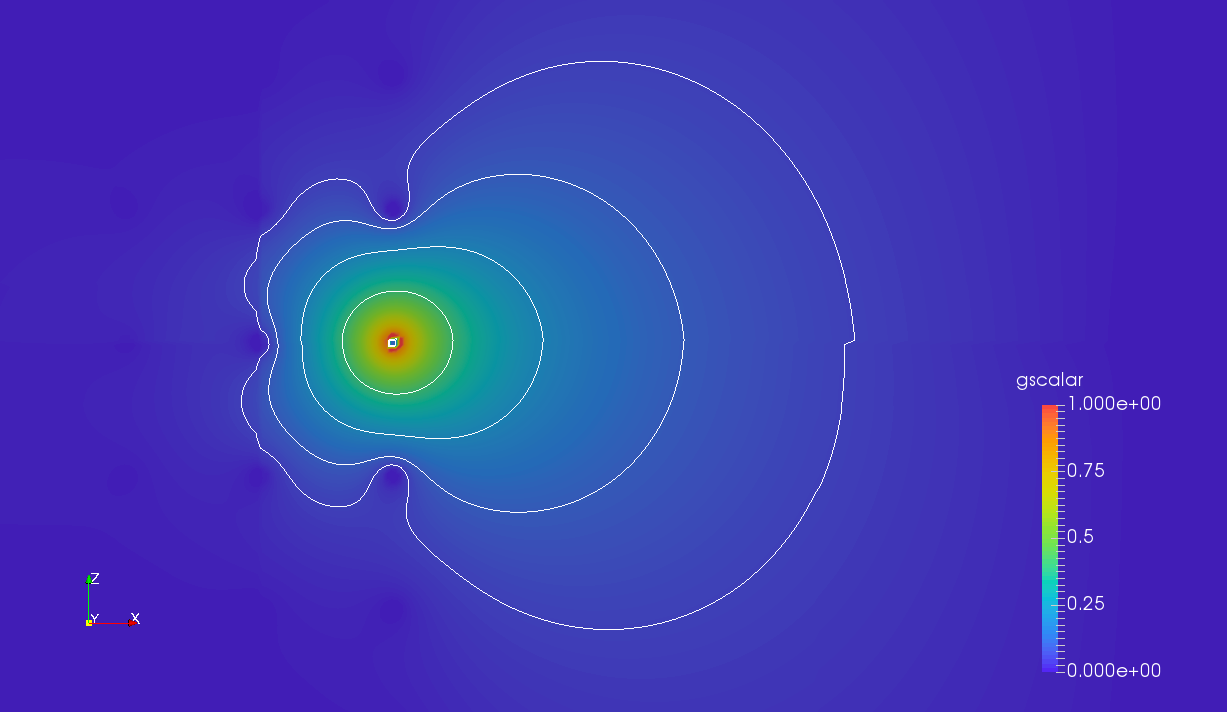
\includegraphics[height=3.5cm]{twodee-fine-u7.png}        
      \end{center}
    \end{column}
    \begin{column}{0.5\textwidth}
      \begin{center}
        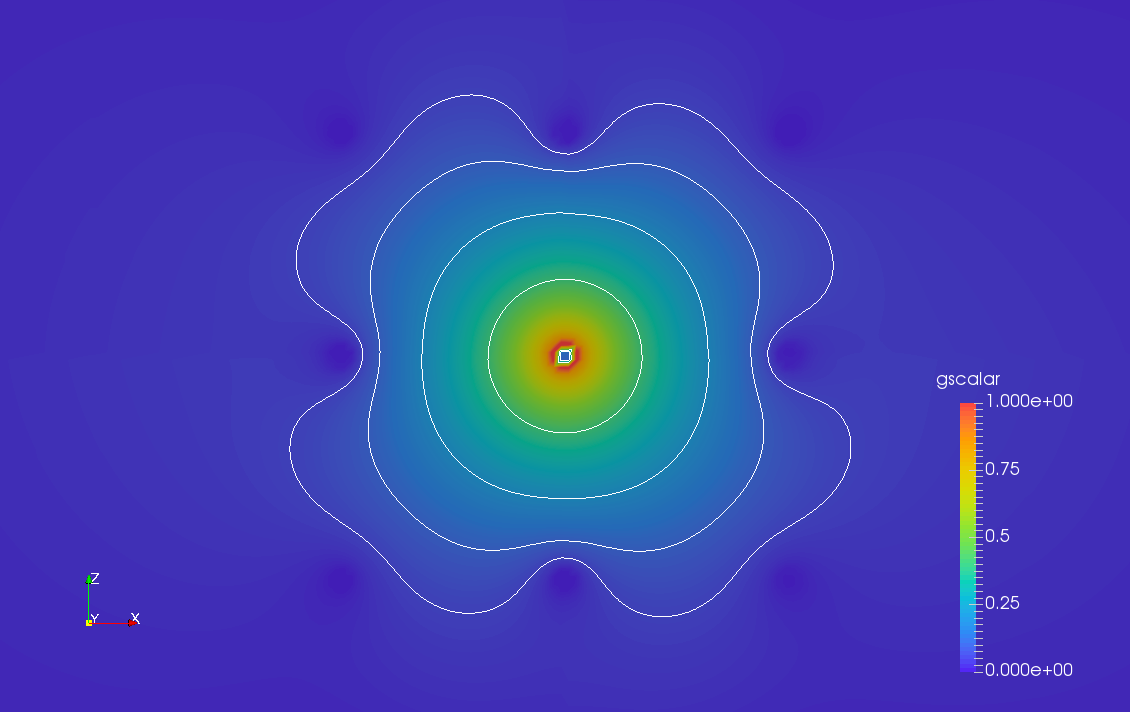
\includegraphics[height=3.4cm]{twodee-fine-v7.png}        
      \end{center}
    \end{column}
  \end{columns}
  \vspace{-1cm}
  \begin{columns}
    \begin{column}{0.5\textwidth}
      \begin{center}
        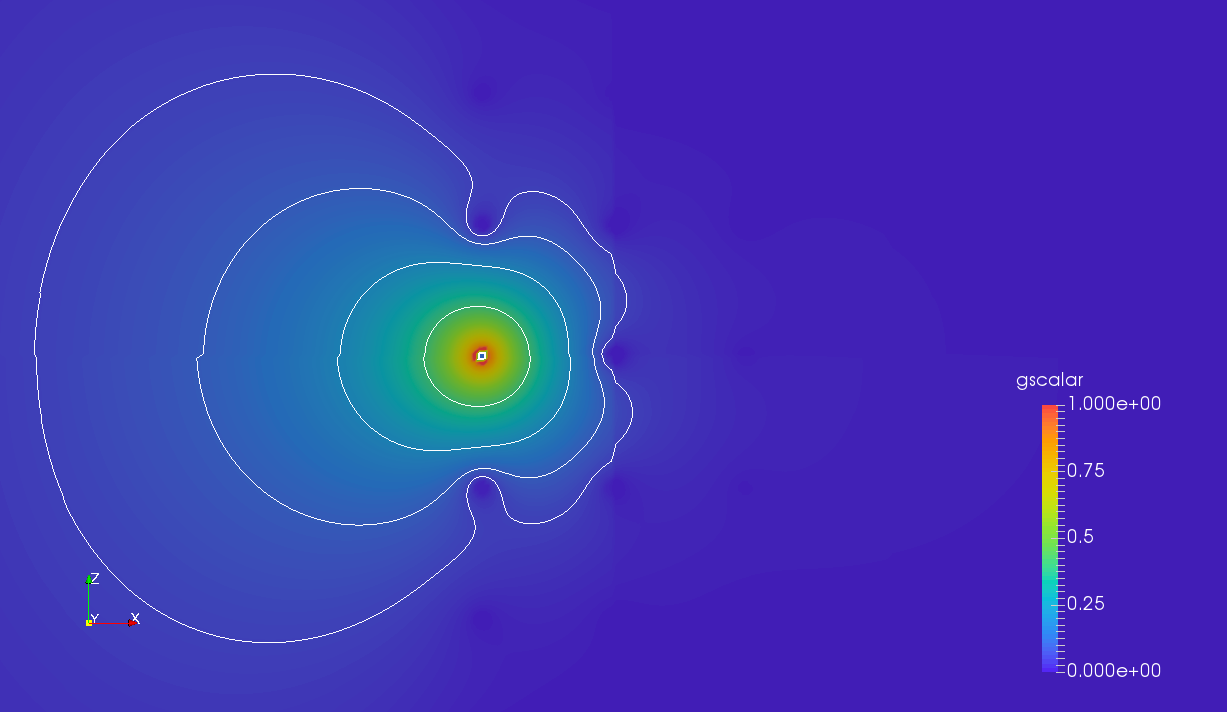
\includegraphics[height=3.5cm]{twodee-fine-w7.png}        
      \end{center}
    \end{column}
    \begin{column}{0.5\textwidth}
      \begin{itemize}\scriptsize
      \item U and W (left) and V (above) planes.
      \item X-Z slices through plane of symmetry.
      \item Lines: 5\%, 10\%, 20\%, 40\% weights.
      \item Initial qualitative agreement with Garfield 2D calculations.
      \item[$\rightarrow$] more exhaustive comparisons needed,
        but satisfactory enough to push on.
      \end{itemize}
    \end{column}
  \end{columns}

\end{frame}



\begin{frame}
  \frametitle{MicroBooNE Geometry Patch}

  \begin{columns}
    \begin{column}{0.5\textwidth}
      \begin{center}
        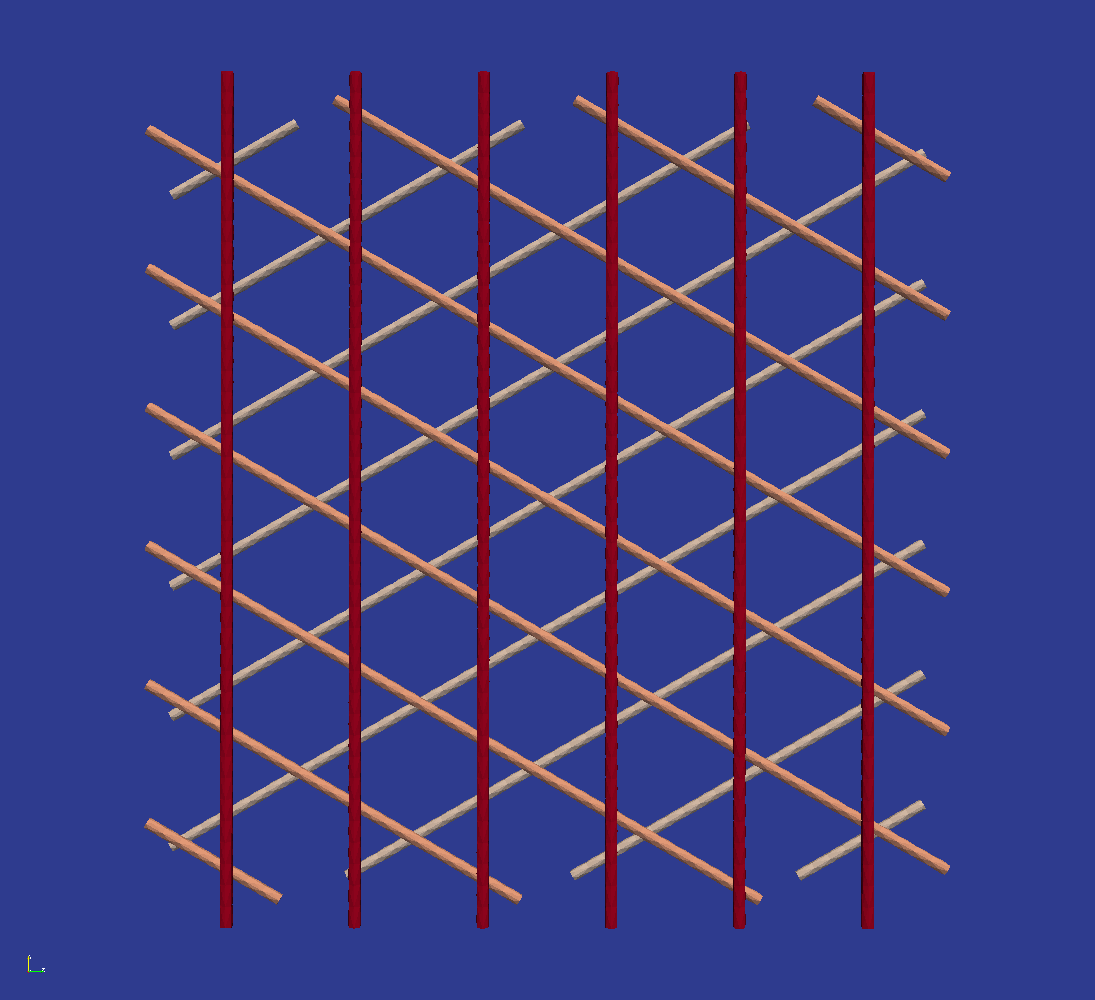
\includegraphics[width=\textwidth]{wires-flat.png}
      \end{center}
    \end{column}
    \begin{column}{0.5\textwidth}
      \begin{center}
        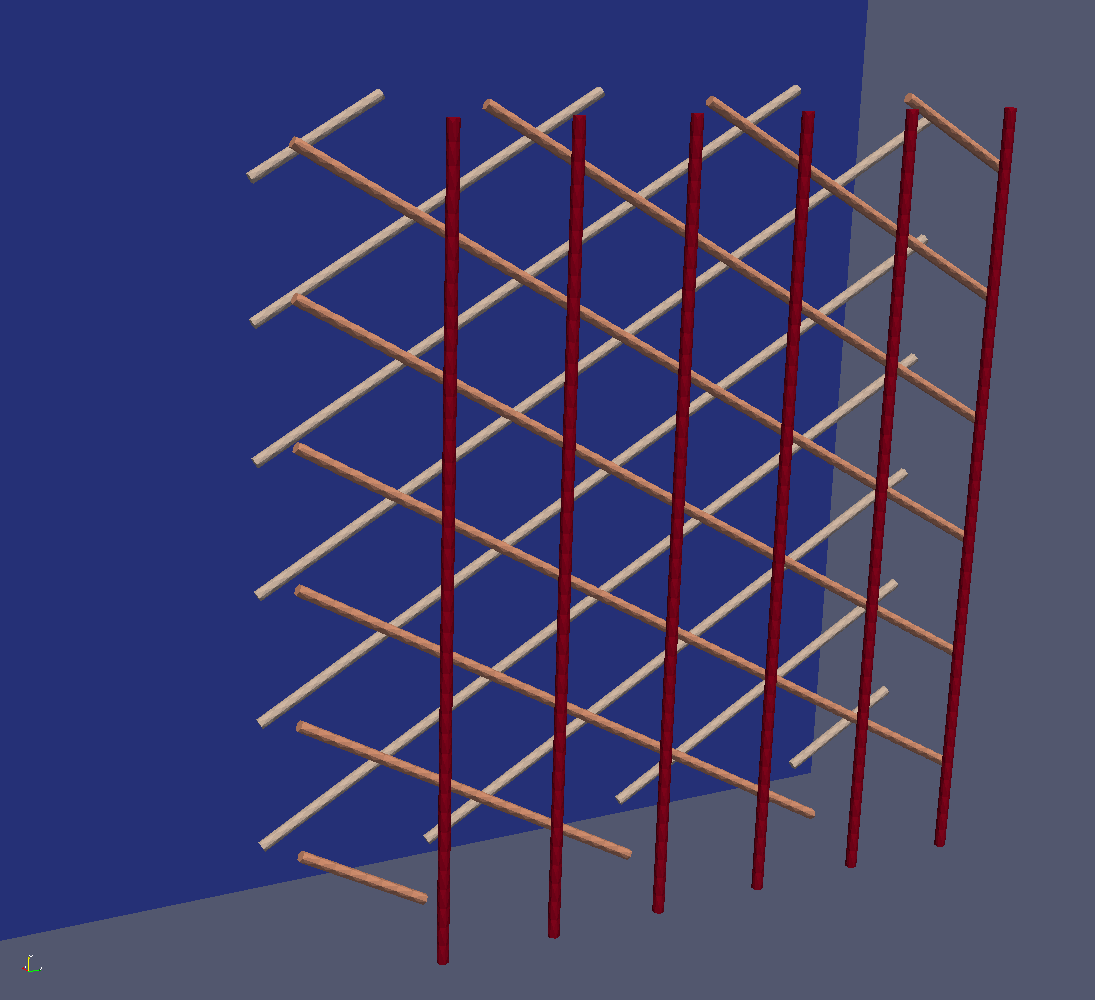
\includegraphics[width=\textwidth]{wires-iso.png}
      \end{center}
    \end{column}
  \end{columns}
  

  \begin{itemize}
  \item Wires parameterized by pitch, angle, bounding box, radius.
  \item Single plane at +20mm for drift potential
  \end{itemize}


\end{frame}

\begin{frame}
  \frametitle{V-plane $\vec{E}_{weight}$ Slices}
  \begin{center}
    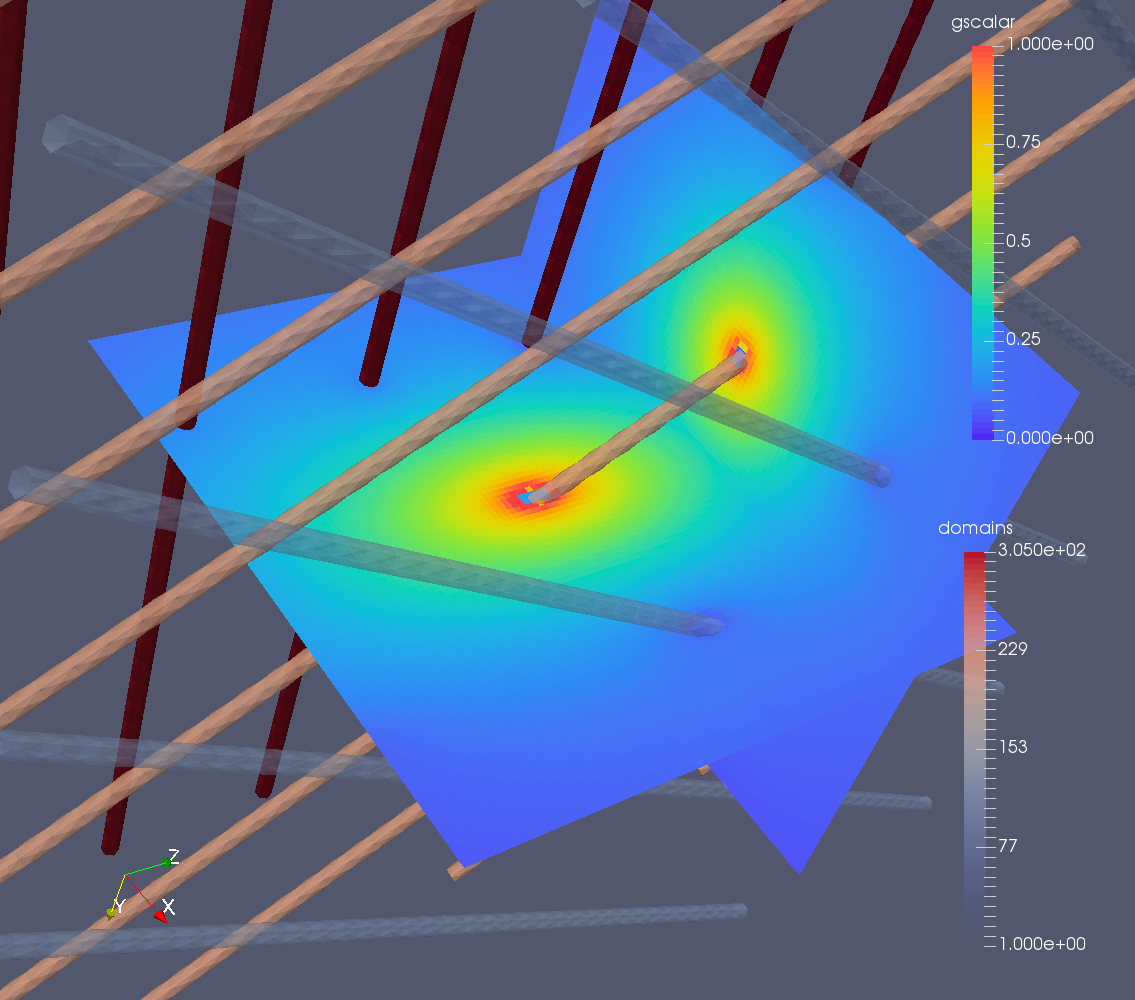
\includegraphics[width=0.6\textwidth]{cap-vweight-field-fine-slices.png}
  \end{center}

  \begin{itemize}\footnotesize
  \item Slices in X-Z and X-Y planes.
  \item Note mismatchs between evaluated voxel grid and wire mesh.
  \end{itemize}
\end{frame}

\begin{frame}{Weighting Potential - 2D vs. 3D wire pattern}

  \vspace{-5mm}

  \begin{columns}
    \begin{column}{0.5\textwidth}
      \begin{center}
        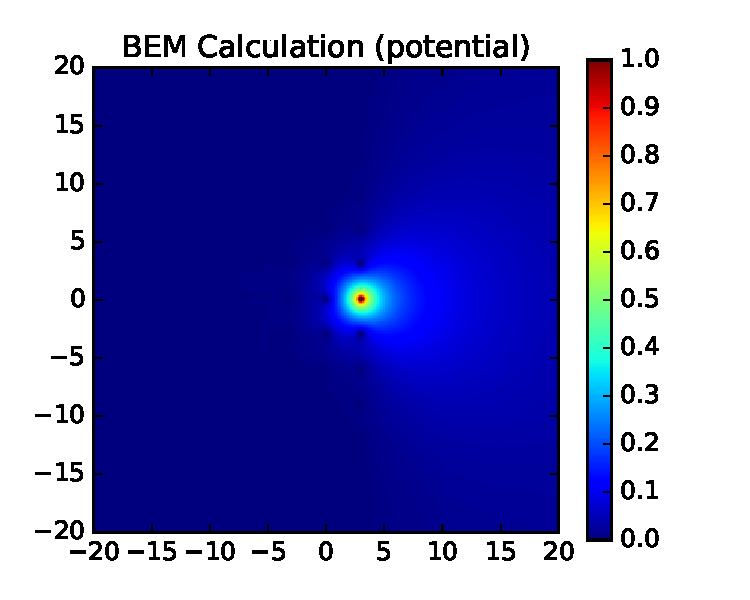
\includegraphics[height=0.65\textheight]{parallel-near-d11.pdf}

        \scriptsize Parallel wires
      \end{center}
    \end{column}
    \begin{column}{0.5\textwidth}
      \begin{center}
        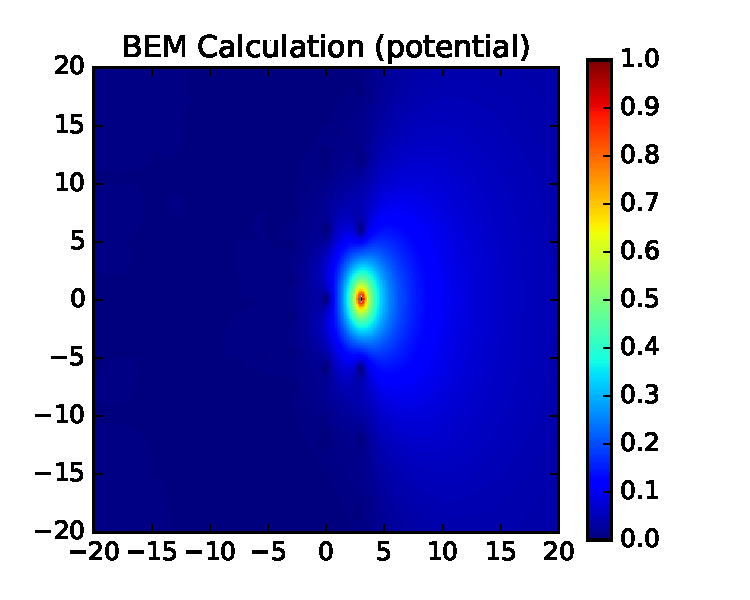
\includegraphics[height=0.65\textheight]{uboone-near-d11.pdf}

        \scriptsize \microboone wires.
      \end{center}
    \end{column}
  \end{columns}

  \begin{center}
    Clear distortion in extent and shape.  Not surprising.
  \end{center}

\end{frame}


\begin{frame}
  \frametitle{Paraview stepping from line source}
  \begin{center}
    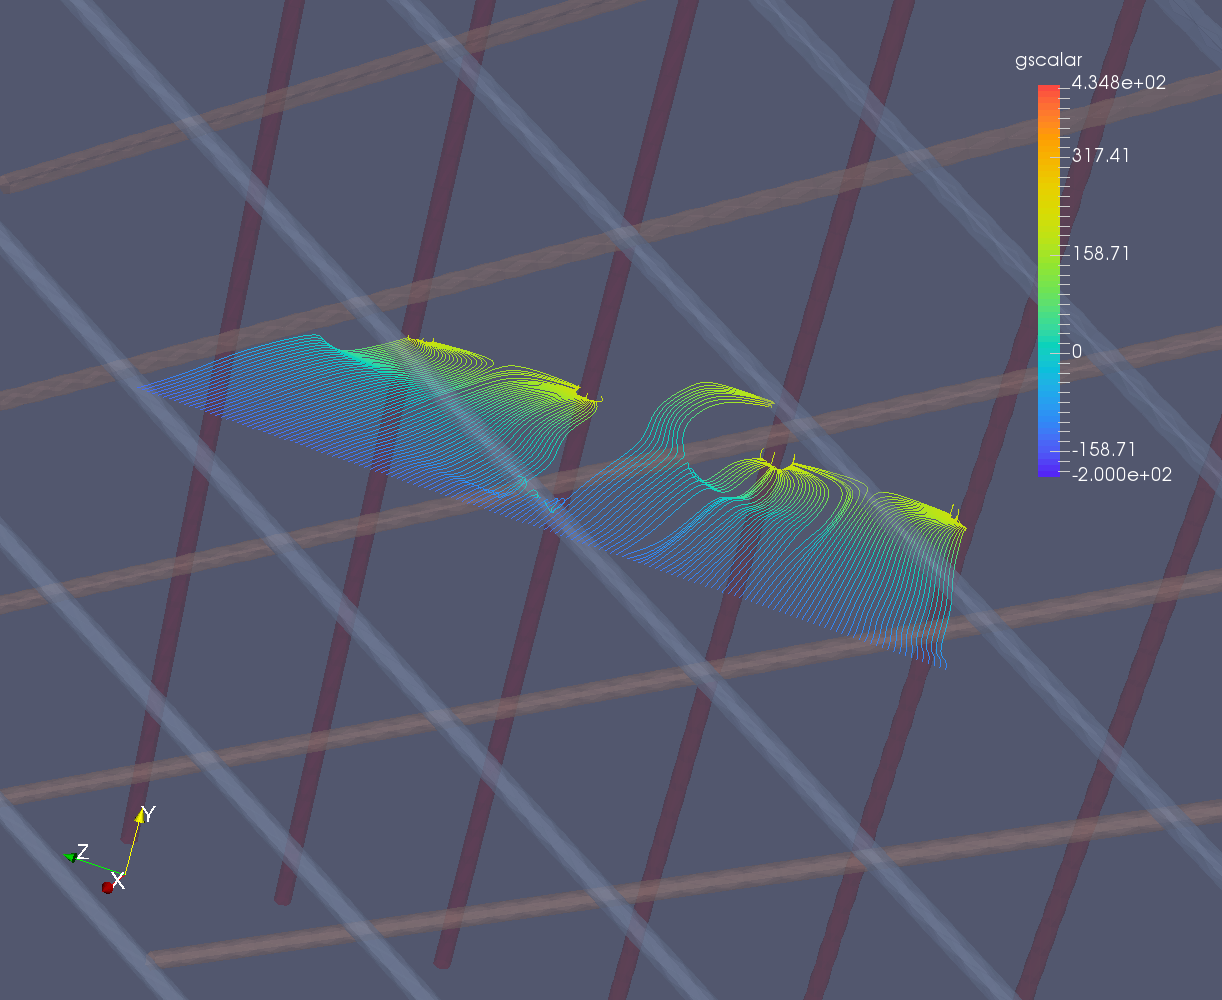
\includegraphics[width=0.6\textwidth]{track-drift-2.png}
  \end{center}

  \begin{itemize}\footnotesize
  \item Line source 2mm in front of U-plane,  paths colored by drift potential.
  \item U-plane transparency violated due to imprecision right near U-wire.
  \end{itemize}

\end{frame}

\begin{frame}
  \frametitle{Initial Response Functions}
  
  \footnotesize

  \begin{center}
    Preliminary and Subject to Change!

    \includegraphics[width=0.3\textwidth]{prec-wresponse-hit.pdf}%
    \includegraphics[width=0.3\textwidth]{prec-uresponse-hit.pdf}%
    \includegraphics[width=0.3\textwidth]{prec-vresponse-hit.pdf}

    Collection and U and V Induction.  Central and nearest neighbor wires.

    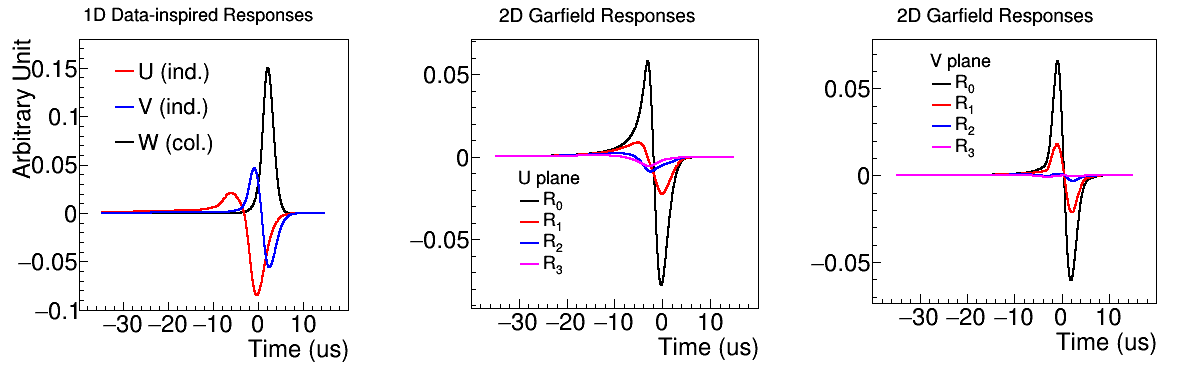
\includegraphics[width=0.7\textwidth]{overall_response.png}

    Data inspired and 2D Garfield calculations.
  \end{center}

\end{frame}

\begin{frame}
  \frametitle{Known Issues Needing Work}
  \begin{enumerate}
  \item Improve precision of fields near wires.
    \begin{itemize}\footnotesize
    \item Voxelization $\to$ \textbf{on-demand sampling} of $\phi_{drift}$ while stepping
    \item Will remove big RAM pig, allow for batch processing.
    \item Gives room for \textbf{finer surface meshing}.
    \end{itemize}
  \item Correct termination of paths.
    \begin{itemize}\footnotesize
    \item Currently, stepping just knows fields (including interiors of wires!)
    \item Must \textbf{terminate stepping} when path ``hits'' a wire.
    \end{itemize}
  \item Explore systematics in response function vs path location.
    \begin{itemize}\footnotesize
    \item Understand \textbf{spatial variations} and properly smooth them.
    \end{itemize}
  \item Limited transverse coverage
    \begin{itemize}\footnotesize
    \item Expect to need $\sim \pm 10$ wires (based on data obs.)
    \item Problem scales somewhere between $N_{wires} \to N^2_{wires}$
    \end{itemize}
  \item uBoone is ``easy first test'', next up:
    \begin{itemize}\footnotesize
    \item DUNE wire crossing pattern
    \item APA edge regions
    \end{itemize}
  \end{enumerate}
\end{frame}

\begin{frame}
  \frametitle{The Software}
  \begin{center}
    \url{https://github.com/brettviren/larf}
  \end{center}

  \begin{itemize}
  \item Expect a name change!
  \item Ready for other users and developers, \textbf{welcome!}
  \item Interfaces: \textbf{simple command line program} or 
    \textbf{Python modules}.
  \item Supports fantastic \textbf{Paraview} visualization app.
  \item Provides various ``management systems'': configuration, data
    storage, result provenance, workflow.
  \end{itemize}

  $\rightarrow$ Warning: \textbf{documentation is trailing code
    development} so let me know if you are interested in
  using/developing and I'll do some freshening.

\end{frame}

\end{document}
%%% Local Variables:
%%% mode: latex
%%% TeX-master: t
%%% End:
